\subsection{Training on merged data} \label{subsec:mergedmodel} 

The first proposed approach is to merge synthetic training data with the real training data into one dataset and use it to train the model. Using this method we have gone through an extensive process of tuning the hyperparameters, similar to what we explained in Section \ref{sec:modelselection}. We have trained more than 50 models and settled on the best-performing one with the following parameters: 

\begin{itemize}
    \setlength\itemsep{1px}
    \item activation function Leaky RELU with a slope of 0.05
    \item batch size of 32
    \item optimizer ADAM with betas = 0.9, 0.999
    \item starting learning rate of $1e^{-3}$
    \item exponential scheduler with $\gamma$ = 0.9
    \item dropout in fully-connected layer with probability of 0.5
    \item L2 regularization with $\lambda$ set to $1e^{-5}$
\end{itemize}

The model was evaluated on the validation set and achieved an accuracy of 94.67 \% on the real data and 99.33 \% on the synthetic data. The training process of the model is depicted in the Figure \ref{fig:lossaccm11}. Comparing this to the final model in Section \ref{subsec:finalmodel} we have improved the performance on the validation set (with real data) significantly. 

\begin{figure}[!h]
\centering
    \begin{subfigure}[t]{.45\textwidth}
        \centering
        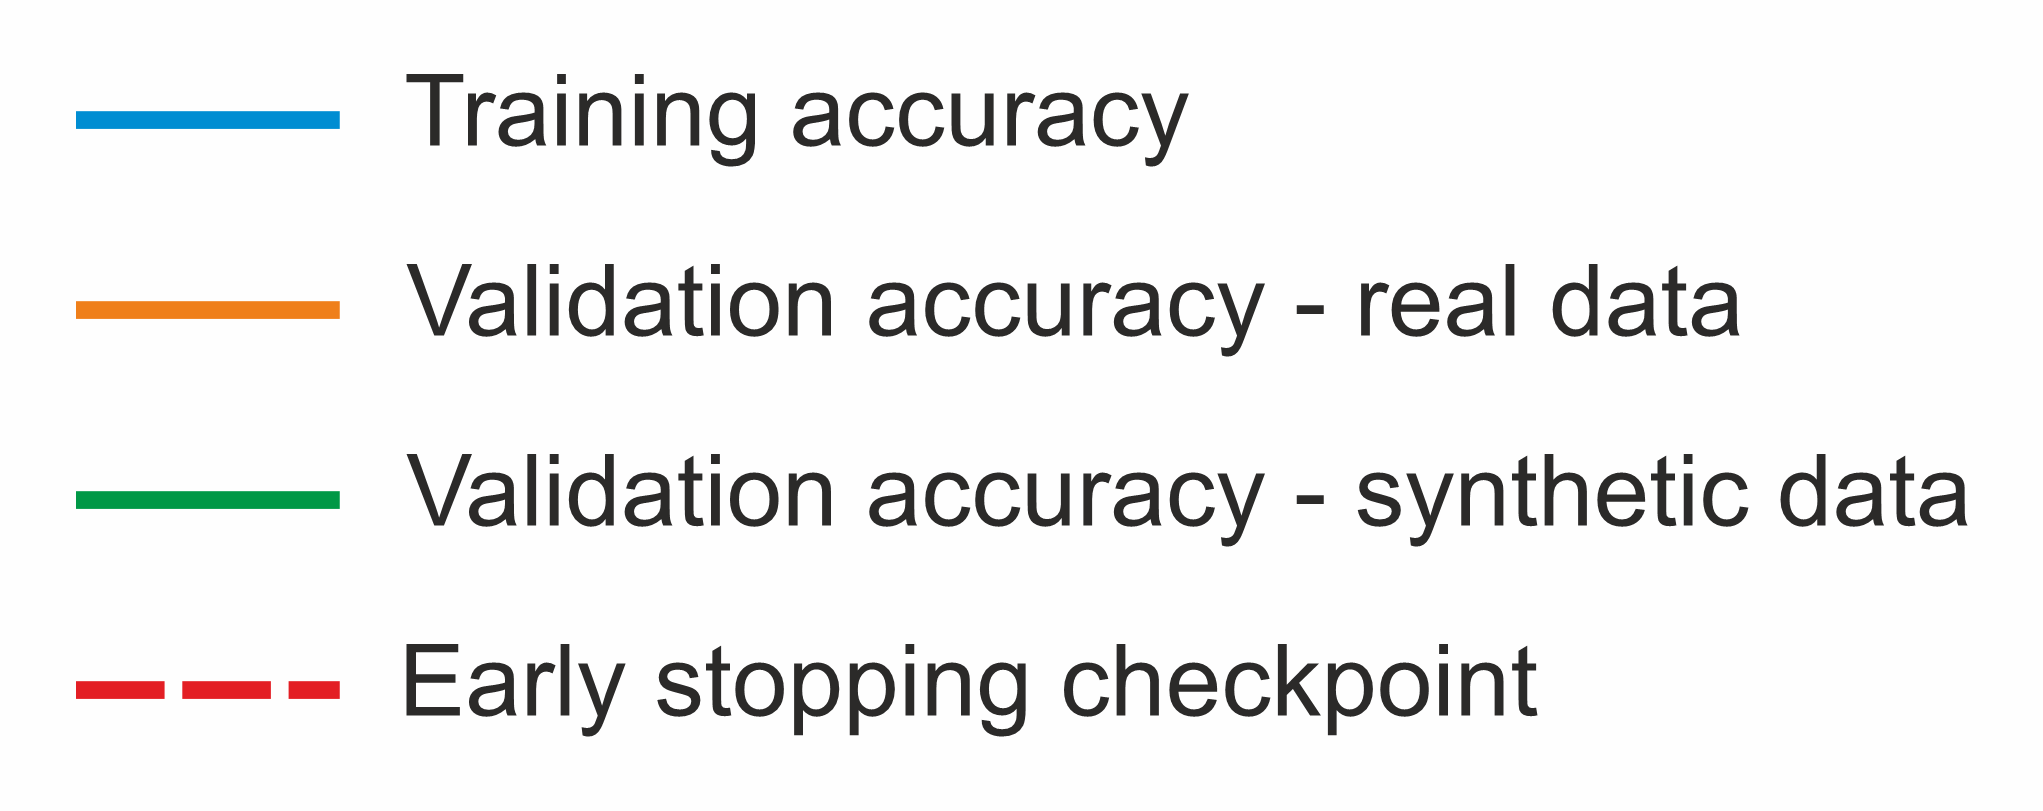
\includegraphics[width=.7\textwidth]{images/popisAc.png}
        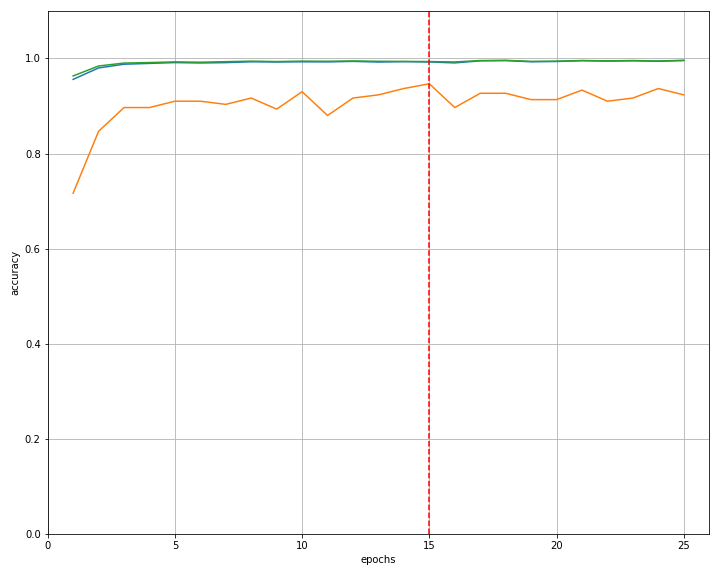
\includegraphics[width=\textwidth]{images/accuracy13r_0.png}
        \caption{The accuracy during training.}
        \label{fig:accm11}
    \end{subfigure}
    \begin{subfigure}[t]{.45\textwidth}
        \centering
        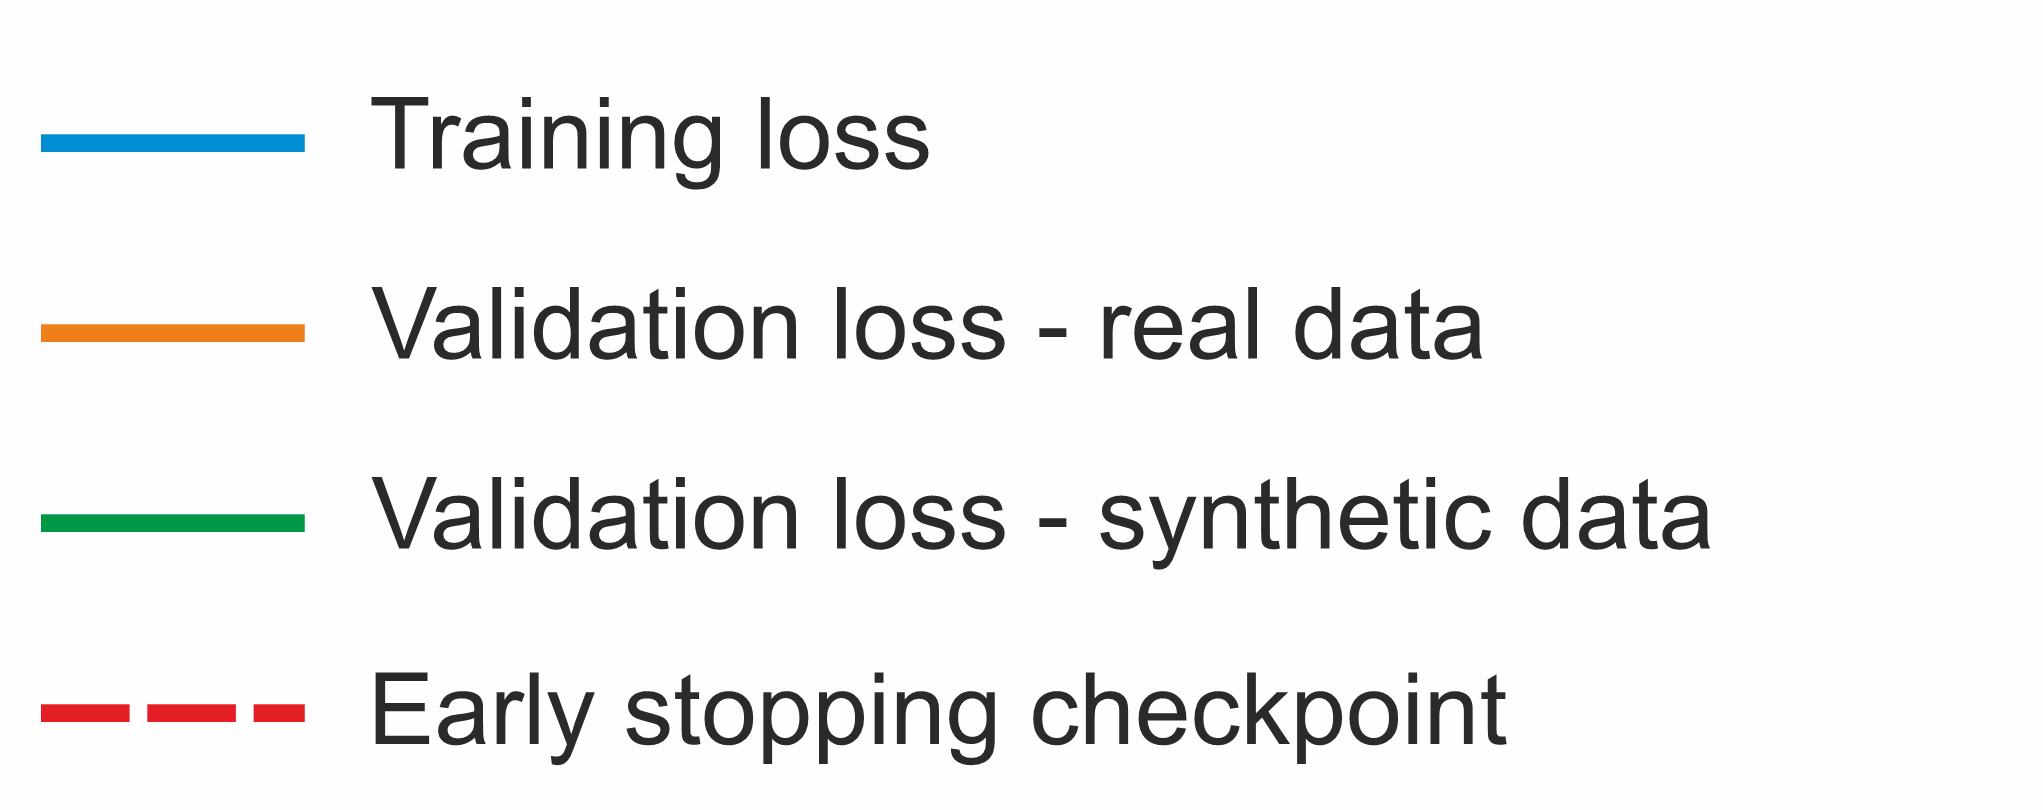
\includegraphics[width=.7\textwidth]{images/popisLoss.png}
        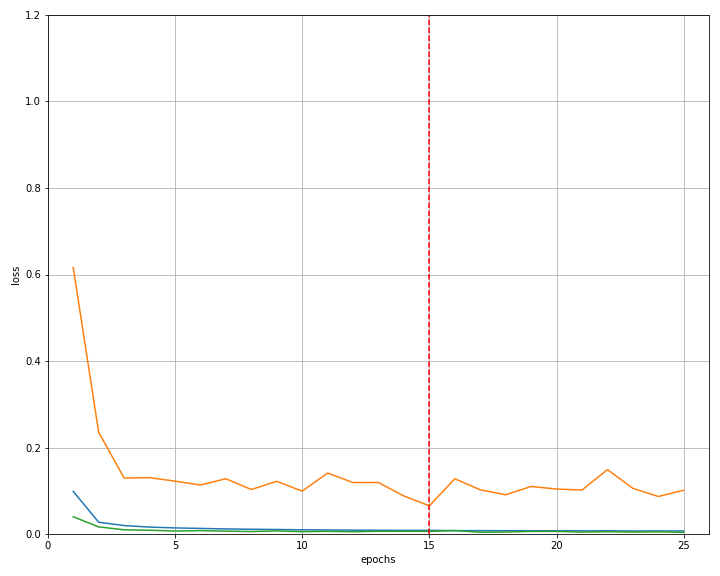
\includegraphics[width=\textwidth]{images/losses13r_0.png}
        \caption{The loss during training.}
        \label{fig:lossm11}
    \end{subfigure}

    \caption{The evolution of the loss and accuracy during training of the model with the merged dataset of real and synthetic images.}
    \label{fig:lossaccm11}
\end{figure}